\documentclass[localFont,alternative]{documentMETADATA}
\usepackage{datetime}
\usepackage{amsmath}
\usepackage{booktabs}

\newdateformat{monthyeardate}{%
  \monthname[\THEMONTH], \THEYEAR}

\def\citNo{2718}
\def\hIndex{27}

\name{Ferdinando}{Fioretto}
\tagline{Assistant Professor}
%\photo{2.5cm}{DCE2small2}
\socialinfo{
	\address{
307 Rice Hall, 
Computer Science,
University of Virginia, 
Charlottesville, VA 22904 - U.S.A.}\\
\personalLink{nandofioretto.com} 
	\email{fioretto@virginia.edu}
	%\smartphone{+1 575 621 5948}
	% \twitter{nandofioretto}
% 	\infos{U.S. Citizen}	
}

\begin{document}

\makecvheader\sloppy\allowdisplaybreaks


	\makecvfooter
		{\textsc{}} %\selectlanguage{english}\today
		{\textsc{Full CV available \link{https://nandofioretto.github.io/assets/cv/cvFioretto.pdf}{\title{here}} }}
		{\thepage}

	% % YAAC Another Awesome CV LaTeX Template
%
% This template has been downloaded from:
% https://github.com/darwiin/yaac-another-awesome-cv
%
% Author:
% Christophe Roger
%
% Template license:
% CC BY-SA 4.0 (https://creativecommons.org/licenses/by-sa/4.0/)
\par{
Développeur et concepteur JEE depuis plusieurs années, j'ai également une expérience de développement sur l'ensemble de l'écosystème Java (Android, J2ME sur PDA et Javacard sur chipset NFC). J'occupe aujourd'hui un poste d'architecte logiciel et reste passionné par mon métier et par les nouvelles technologies en général. Particulièrement intéressé par les nouveaux usages  et les opportunités que peut amener le développement de la 4G sur le territoire, je souhaite poursuivre ma carrière sur des projets de développement mobile innovants en qualité d'architecte logiciel et/ou développeur/concepteur.
}                % Research Statement

	\begin{tabular}{r l} 
	{\bf Research Interests:} &
	{Machine Learning}~|~
	%{Optimization}~|~
	% {Responsible AI}~|~
	{Differential Privacy}~|~
	{Algorithmic Fairness}~|~
	{AI for Science and Engineering}
%	{Differentiable Optimization}~|~
	%{Power Systems}.
	\end{tabular}

%Education and Training, 
% Research and Professional Experience, 
% Collaborations and Affiliations, Publications and Synergistic Activities

\sectionTitle{Education and Training}{}%{\faSuitcase}
\vspace{-6pt}
\begin{experiences}
  \job
    {Sep.~2018}{Dec.~2019}
    {Georgia Institute of Technology}
    {School of Industrial and System Engineering}
    {Atlanta, GA}
    {Post-doctoral Researcher}\\[-10pt]
  \job
    {Sep.~2016}{Dec.~2018}
    {University of Michigan}
    {Industrial and Operations Engineering}
    {Ann Arbor, MI}
    {Research Fellow}
  \job
    {}{Aug.~2016}
    {University of Udine}%\footnote{Dual degree with New Mexico State University}}
    {Computer Science}
    {Udine, IT}
    {Ph.D.~in Computer Science (with MS in 2012)}
  \job
    {}{Nov.~2009}
    {University of Parma}{Computer Science \& Mathematics}
    {Parma, IT}
    {BS.~in Computer Science}
\end{experiences}

\vspace{-2pt}
\sectionTitle{Research and Professional Experience}{}%{\faSuitcase}
\vspace{-6pt}
\begin{experiences}
  \job
    {Jun.~2023}{Current}
    {University of Virginia}{Computer Science}
    {Charlottesville, VA}
    {Assistant Professor}\\[-10pt]
  \job
    {Jan.~2020}{Jun.~2023}
    {Syracuse University}{Electrical Engineering \& Computer Science}
    {Syracuse, NY}
    {Assistant Professor}
\end{experiences}

\vspace{-6pt}
\sectionTitle{Selected Honors and Awards}{}%{\faMortarBoard}
\vspace{-6pt}

\begin{awards}
	\awardentry
	{2024}
	{Outstanding Research Faculty Award}
	{University of Virginia}% at the Annual Research Achievement Awards}
	{https://research.virginia.edu/initiatives/research-achievement-awards/2024-research-award-winners}
	{Link}

	\awardentry
	{2022}
	{Caspar Bowden PET Award}%{IJCAI}
	{Privacy Enhancing Technologies (PETs)}
	{https://petsymposium.org/award/winners.php}
	{Link}

	\awardentry
	{2022}
	{NSF CAREER Award}{National Science Foundation}
	{https://ecs.syracuse.edu/about/news/electrical-engineering-and-computer-science-professor-ferdinando-fioretto-receives-national-science-foundation-nsf-career-award}
	{Press}
	% {https://www.nsf.gov/awardsearch/showAward?AWD_ID=2143706}
	% {Link}

	\awardentry
	{2022}
	{Google Research Scholar Award}{Google}
	{https://research.google/outreach/research-scholar-program/recipients/}
	{Link}
	%  "Equity of Differentially Private Decision Processes," to our Google Research Scholar program

	\awardentry
	{2022}
	{Amazon Research Award}{Amazon -- AWS AI}
	{https://www.amazon.science/research-awards/program-updates/fall-2021-and-winter-2022-amazon-research-awards-recipients-announced}
	{Link}

	\awardentry
	{2022}
	{Best Paper Award}{IEEE Transaction of Power System}
	{https://ieeexplore.ieee.org/document/9729673}{Link}

	\awardentry
	{2022}
	{Early Career Spotlight}%{IJCAI}
	{International Joint Conference on Artificial Intelligence (IJCAI)}
	{https://ijcai-22.org/}
	{Link}

	\awardentry
	{2021}
	{Early Career Researcher Award}
	{Association for Constraint Programming}
	{https://www.a4cp.org/awards/early-career-research-award}
	{Link}
	% {For contribution to constraint programming and, in particular,
	% fundamental advances in distributed constraint satisfaction, constraint-based
	% differential privacy, fairness in artificial intelligence, and their 
	% applications in energy, mobility, and census data.}

	\awardentry
	{2021}
	{Mario Gerla Young Investigator Award for Research in Computer Science}{ISSNAF}
	{https://ambwashingtondc.esteri.it/ambasciata_washington/en/sala-stampa/dall_ambasciata/issnaf-awards-2021-ecco-i-migliori.html}
	{Press}

	% \awardentry
	% {2021}
	% {Outstanding Reviewer Award}%{NeurIPS}
	% {Conference on Neural Information Processing Systems (NeurIPS)} 
	% {https://nips.cc/Conferences/2021/}{Link}
		
	\awardentry
	{2021}
	{Best Paper Award}{IEEE Transaction of Power System}
	{https://ieeexplore.ieee.org/stamp/stamp.jsp?tp=\&arnumber=9358108}{Link}
	%{Assigned to seven out of all IEEE-TPS papers published in 2018--2020.}

	\awardentry
	{2018}
	{Best AI Dissertation Award}{AI*IA} % The Italian Association for Artificial Intelligence (AI*IA)
	{https://sites.google.com/a/aixia.it/vincitori-premi/Home}{Press}

	% \awardentry
	% {2017}
	% {Most Visionary Workshop Paper Award}{International Conference of 
	% Autonomous Agents and Multiagent Systems (AAMAS)}
 %   {https://link.springer.com/book/10.1007/978-3-319-71679-4}{Link}

	% \awardentry
	% {2013}
	% {Best Student Paper Award}{Computational Methods in System Biology (CMSB)}
	% {https://www2.ist.ac.at/cmsb13/program/}{Link}
\end{awards}	


\sectionTitle{Selected Publications}{}%{\faBook}

\begin{keywords}
\keywordsentry{\textbf{Summary}:}
{			 \faAngleRight~ \nemph{77} Conference papers
\hspace{4pt} \faAngleRight~ \nemph{14} Journals articles
\hspace{4pt} \faAngleRight~ \nemph{2} Book chapters
\hspace{4pt} \faAngleRight~ \nemph{3} Editorial articles
		 \\& \faAngleRight~ \nemph{31} Workshop papers
\hspace{4pt} \faAngleRight~ \nemph{20+} Preprints
}
\keywordsentry{\textbf{Total citations}:}
{\citNo \hspace{8pt} 
 \textbf{H-index}: \hIndex \hspace{8pt} 
 \gscholar{Google Scholar} 
 %\textbf{CS-rankings [from 2019]:} \nemph{12} (count)
 }% \faExternalLink}} 
\end{keywords}
%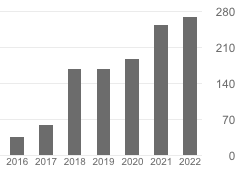
\includegraphics[height=30pt]{scholar-cit.png}

{\textsc{Full Publication list available \link{https://scholar.google.com/citations?user=ASf9Q04AAAAJ&hl=en}{\title{here}} }}
\begin{pubs}

\confentryShort
	{1}
	{{Vincenzo Di Vito}, Mostafa Mohammadian, Kyri Baker, {\bf Ferdinando Fioretto}}
	{Learning To Solve Differential Equation Constrained Optimization Problems}
	{\procICLR, 2025}
	{https://arxiv.org/abs/2410.01786}

\confentryShort
	{2}
	{{Jacob K.~Christopher}, {Michael Cardei}, Brian R Bartoldson, Bhavya Kailkhura, {\bf Ferdinando Fioretto}}
	{Speculative Diffusion Decoding: Accelerating Language Generation through Diffusion}
	{\procNAACL, 2025}
	{https://arxiv.org/abs/2408.0563605246}

\confentryShort
	{3}
	{{\bf Ferdinando Fioretto}, Diptangshu Sen, Juba Ziani}
	{Differentially Private Data Release on Graphs: Inefficiencies and Unfairness}
	{\procAISTATS, 2025}
	{https://arxiv.org/abs/2408.05246}

\confentryShortAwd
	{4}
	{{Joonhyuk Ko}, Juba Ziani, {Saswat Das}, Matt Williams, {\bf Ferdinando Fioretto}}
	{Fairness Issues and Mitigations in (Differentially Private) Socio-demographic Data Processes}
	{\procAAAI, 2025}
	{https://arxiv.org/abs/2408.08471}
	{Oral}

\confentryShort
	{5}
	{Khang Tran, {\bf Ferdinando Fioretto}, Issa Khalil, My T.~Thai, NhatHai Phan}
	{FairDP: Certified Fairness with Differential Privacy}
	{In \venue{IEEE Secure and Trustworthy Machine Learning Conference (SaTML 2025)}, 2025}
	{https://arxiv.org/abs/2305.16474}

% 2024 ------
\confentryShort
	{6}
	{Jacob K Christopher and {\bf Ferdinando Fioretto}}
	{Constrained Synthesis with Projected Diffusion Models}
	{\procNeurIPS, 2024}
	{https://arxiv.org/abs/2402.03559}

\confentryShortAwd
	{7}
	{Jacob K.~Christopher, Michael Cardei, Brian R Bartoldson, Bhavya Kailkhura, {\bf Ferdinando Fioretto}}
	{Speculative Diffusion Decoding: Accelerating Language Generation through Diffusion}
	{\procNeurIPS, 2024}
	{https://arxiv.org/abs/2408.05636}
	{Oral at AI4Mat Workshop}

\confentryShort
	{8}
	{Sree Nelaturu, N.~Ravichandran, Cuong Tran, Sara Hooker, and {\bf Ferdinando Fioretto}}
	{On The Fairness Impacts of Hardware Selection in Machine Learning}	
	{\procICML, 2024}
	{https://arxiv.org/abs/2312.03886}

\confentryShort
	{9}
	{Saswat Das, Marco Romanelli, {\bf Ferdinando Fioretto}}
	{Disparate Impact on Group Accuracy of Linearization for Private Inference}
	{\procICML, 2024}
	{https://arxiv.org/abs/2402.03629}
	
\confentryShort
	{10}
	{My H.~Dinh, James Kotary, {\bf Ferdinando Fioretto}}
	{End-to-End Learning for Fair Multiobjective Optimization Under Uncertainty}
	{\procUAI, 2024}
	{https://arxiv.org/abs/2402.07772}

\confentryShort
	{11}
	{Ethan King, {James Kotary}, {\bf Ferdinando Fioretto}, Jan Drgona}
	{Metric Learning to Accelerate Convergence of Operator Splitting Methods for Differentiable Parametric Programming}
	{\venue{63rd IEEE Conference on Decision and Control (CDC)}, 2024}
	{https://arxiv.org/abs/2404.00882}

\confentryShort
	{12}%{ArXiv}
	{Cuong Tran, Keyu Zhu, Pascal Van Hentenryck, {\bf Ferdinando Fioretto}}
	{Fairness Increases Adversarial Vulnerability}
	{\procIJCAI, 2024}
	{https://arxiv.org/abs/2211.11835}

\confentryShort
	{13}
	{{James Kotary}, {Vincenzo Di Vito}, {Jacob K.~Christopher}, Pascal Van Hentenryck, Ferdinando Fioretto}
	{Predict-Then-Optimize by Proxy: Learning Joint Models of Prediction and Optimization}
  {\procECAI, 2024}
  {https://arxiv.org/2311.13087}

\confentryShort
	{7}
	{My H.~Dinh, James Kotary, {\bf Ferdinando Fioretto}}
	{Learning Fair Ranking Policies via Differentiable Optimization of Ordered Weighted Averages}
	{\procFAccT, 2024}
	{https://arxiv.org/abs/2402.05252}

\confentryShort
	{8}
	{{\bf Ferdinando Fioretto}, Keyu Zhu, Pascal Van Hentenryck, Saswat Das, Christine Task}
	{Finding $\epsilon$ and $\delta$ of Traditional Disclosure Control Systems}
	{\procAAAI, 2024}
	{https://arxiv.org/abs/2301.12204}

\confentryShort
	{9}
	{{Cuong Tran} and {\bf Ferdinando Fioretto}}
	{Data Minimization at Inference Time}
	{\procNeurIPS, 2023}
	{https://arxiv.org/abs/2305.17593}

\confentryShort
	{10}
 	{Vladimir Dvorkin and {\bf Ferdinando Fioretto}}
	{Price-Aware Deep Learning for Electricity Markets}
	{\venue{Tackling Climate Change with Machine Learning, at NeurIPS}, 2023}
	{https://arXiv.org/abs/2308.01436}

\confentryShort 
	{11} %{IJCAI}
	{{James Kotary}, {My H.~Dinh}, {\bf Ferdinando Fioretto}}
	{Folded Optimization for End-to-End Model-Based Learning}
	{\procIJCAI, 2023}
	{https://arxiv.org/abs/2301.12047}

\confentryShort
 {12} %{IJCAI}
	{{James Kotary}, {Vincenzo Di Vito}, {\bf Ferdinando Fioretto}, Pascal Van Hentenryck}
	{SF-PATE: Scalable, Fair, and Private Aggregation of Teacher Ensembles}
  {\procIJCAI, 2023}
	{https://arxiv.org/abs/2204.05157}

\confentryShort
  {13} %{IJCAI}
	{{James Kotary}, {Vincenzo Di Vito}, {\bf Ferdinando Fioretto}}
	{End-to-End Combinatorial Ensemble Learning}
  {\procIJCAI, 2023}
	{http://arxiv.org/abs/2211.00251}

\confentryShort
  {14} %{IJCAI}
	{{Cuong Tran}, {\bf Ferdinando Fioretto}}
	{On the Fairness Impacts of Private Ensembles Models}
    {\procIJCAI, 2023}
	{http://arxiv.org/abs/2109.08630}

\confentryShort
	{15} %{PES}
	{Terrence W.K. Mak, {\bf Ferdinando Fioretto}, Pascal Van Hentenryck}
	{Load Encoding for Learning AC-OPF}
	{Proceedings of the \venue{IEEE PES General Meeting (PES)}, 2023}
	{https://arxiv.org/abs/2101.03973}

\confentryShort
	{16}
	{{My H.~Dinh}, {\bf Ferdinando Fioretto}, Mostafa Mohammadian, and Kyri Baker}
	{An Analysis of the Reliability of AC Optimal Power Flow Deep Learning Proxies}
	{\venue{IEEE PES Innovative Smart Grid Technologies}, 2023}
	{https://arxiv.org/abs/2111.11168}

\confentryShort
  {17} %{AAMAS}
	{{James Kotary}, {Vincenzo Di Vito}, {\bf Ferdinando Fioretto}}
	{End-to-End Optimization and Learning for Multiagent Ensembles}
    {\procAAMAS, 2023}
	{http://arxiv.org/abs/2211.00251}

\confentryShortAwd
	{18} %{NeurIPS}
	{{Cuong Tran}, {\bf Ferdinando Fioretto}, Jung-Eun Kim, {Rakshit Naidu}}
	{Pruning has a disparate impact on model accuracy}
	{\procNeurIPS, 2022}
	{http://arxiv.org/abs/2205.13574}
	{Spotlight}

	\confentryShort
	{19} %{IJCAI}
	{Keyu Zhu, {\bf Ferdinando Fioretto}, Pascal Van Hentenryck}
	{Post-processing of Differentially Private Data: A Fairness Perspective}
	{\procIJCAI, 2022}
	{http://arxiv.org/abs/2202.09425}	

	\confentryShort
	{20} %{IJCAI}
	{{\bf Ferdinando Fioretto}, {Cuong Tran}, Keyu Zhu, Pascal Van Hentenryck}
	{Differential Privacy and Fairness in Decisions and Learning Tasks: A Survey}
	{\procIJCAI, 2022}
	{http://arxiv.org/abs/2202.08187}	

	\confentryShortAwd
	{21} %{IJCAI}
	{{\bf Ferdinando Fioretto}}
	{Integrating Machine Learning and Optimization to Boost Decision Making}
	{\procIJCAI, 2022}
	{https://web.ecs.syr.edu/~ffiorett/files/papers/Fioretto-IJCAI22-EC.pdf}	
	{Early Career Spotlight}

	\confentryShort
	{22} %{WWW}
	{{James Kotary}, {\bf Ferdinando Fioretto}, Pascal Van Hentenryck, Ziwei Zhu}
	{End-to-end Learning for Fair Ranking Systems}
	{\procWWW, 2022}
	{http://arxiv.org/abs/2111.10723}	
	
	\confentryShort
	{23} %{AAAI} 
	{{James Kotary}, {\bf Ferdinando Fioretto}, Pascal Van Hentenryck}
	{Fast Approximations for Job Shop Scheduling: A Lagrangian Dual Deep Learning Method}
	{\procAAAI, 2022}
	{http://arxiv.org/abs/2110.06365}

	\confentryShort
	{24} %{PMAPS}
	{Lesia Mitridati, Emma Romei, Gabriela Hug, {\bf Ferdinando Fioretto}}
	{Differentially-Private Heat and Electricity Markets Coordination}
	{\procPMAPS, 2022}
	{https://arxiv.org/abs/2201.10634}

	\confentryShort
	{25} %{PMAPS}
	{Mostafa Mohammadian, Kyri Baker, {My H.~Dinh}, {\bf Ferdinando Fioretto}}
	{Learning Solutions for Intertemporal Power Systems Optimization with Recurrent Neural Networks}
	{\procPMAPS, 2022}
	{https://ieeexplore.ieee.org/document/9810638}

	\confentryShort 
	{26} %{NeurIPS}
	{{Cuong Tran}, {My H.~Dinh}, {\bf Ferdinando Fioretto}}
	{Differentially Private Deep Learning under the Fairness Lens}
	{\procNeurIPS, 2021}
	{https://arxiv.org/pdf/2106.02674.pdf}

	\confentryShort 
	{27} %{NeurIPS}
	{{James Kotary}, {\bf Ferdinando Fioretto}, Pascal Van Hentenryck}
	{Learning Hard Optimization Problems: A Data Generation Perspective}
	{\procNeurIPS, 2021}
	{https://arxiv.org/pdf/2106.02674.pdf}

	\confentryShortAwd 
	{28} %{IJCAI}
	{{Cuong Tran}, {\bf Ferdinando Fioretto}, Pascal Van Hentenryck, {Zhiyan Yao}}
	{Decision Making with Differential Privacy under the Fairness Lens}
	{\procIJCAI, 560--566, 2021}
	{https://www.ijcai.org/proceedings/2021/78}
	{2022 Caspar Bowden PET Award}

	\confentryShort 
	{29} %{IJCAI}
	{{James Kotary}, {\bf Ferdinando Fioretto}, Pascal Van Hentenryck, Bryan Wilder}
	{End-to-End Constrained Optimization Learning: A Survey}
	{\procIJCAI, 4475--4482, 2021}
	{https://www.ijcai.org/proceedings/2021/610}

	\confentryShort 
	{30} %{AAAI}
	{Keyu Zhu, Pascal Van Hentenryck, {\bf Ferdinando Fioretto}}
	{Bias and Variance of Post-processing in Differential Privacy}
	{\procAAAI, 11177--11184, 2021}
	{https://ojs.aaai.org/index.php/AAAI/article/view/17333}

	\confentryShort 
	{31} %{AAAI}
	{{Cuong Tran}, {\bf Ferdinando Fioretto}, Pascal Van Hentenryck}
	{Differentially Private and Fair Deep Learning: A Lagrangian Dual Approach}
	{\procAAAI, 9932--9939, 2021}
	{https://ojs.aaai.org/index.php/AAAI/article/view/17193}


	\confentryShort
	{32} %{ECML}
	{{\bf Ferdinando Fioretto}, Pascal Van Hentenryck, Terrence W.K. Mak, {Cuong Tran}, Federico Baldo, Michele Lombardi} 
	{A Lagrangian Dual Framework for Deep Neural Networks with Constraints}
	{\procECML, 18--135, 2020}
	{https://arxiv.org/abs/2001.09394}

	\confentryShort
		{33} %{IJCAI}
		{{\bf Ferdinando Fioretto}, Lesia Mitridati, Pascal Van Hentenryck}
		{Differential Privacy Stackebelg Games}
		{\procIJCAI, 3480--3486, 2020}
		{https://www.ijcai.org/proceedings/2020/0481.pdf}

	\confentryShortAwd
		{34} %{IJCAI}
		{{\bf Ferdinando Fioretto}, Pascal Van Hentenryck}
		{OptStream: Releasing Time Series Privately}
		{\procIJCAI, 5135--5139, 2020}
	  {https://www.ijcai.org/proceedings/2020/722}
	  {Invited journal paper}
	
	\confentryShort
		{35} %{PSCC}
		{Terrence W.K.~Mak, {\bf Ferdinando Fioretto}, Pascal Van Hentenryck}
		{Privacy-Preserving Obfuscation for Distributed Power Systems}
		{\procPSCC, 2020}
		{https://arxiv.org/abs/1910.04250}

	\confentryShort
		{36} %{AAAI}
		{{\bf Ferdinando Fioretto}, Terrence W.K.~Mak, Pascal Van Hentenryck}
		{Predicting AC Optimal Power Flows: Combining Deep Learning and Lagrangian Dual Methods}
	  	{\procAAAI, pages 630--637, 2020}
	  	{https://ojs.aaai.org//index.php/AAAI/article/view/5403}

	\confentryShort
		{37} %{PRIMA}
	    {Atena Tabakhi, William Yeoh, {\bf Ferdinando Fioretto}}
	    {The Smart Appliance Scheduling Problem: A Bayesian Optimization Approach}
	    {\procPRIMA, 100--115, 2020}
	    {https://link.springer.com/chapter/10.1007\%2F978-3-030-69322-0\_7}


	\confentryShort
		{38} %{AAMAS}
		{{\bf Ferdinando Fioretto}, Pascal Van~Hentenryck}
		{Privacy-Preserving Federated Data Sharing}
	  	{\procAAMAS, pages 638--646, 2019}
	  	{https://dl.acm.org/doi/abs/10.5555/3306127.3331750}

	\confentryShort
		{39} %{IJCAI}
		{{\bf Ferdinando Fioretto}, Terrence W.K.~Mak, Pascal Van Hentenryck}
		{Privacy-Preserving Obfuscation of Critical Infrastructure Networks}
	  	{\procIJCAI, pages 1086--1092, 2019}
	  	{https://www.ijcai.org/proceedings/2019/0152.pdf}

	\confentryShortAwd
		{40} %{CP}
		{{\bf Ferdinando Fioretto}, Pascal Van Hentenryck}
		%\href{https://web.ecs.syr.edu/~ffiorett/files/papers/cp19.pdf}
		{Differential Privacy of Hierarchical Census Data: An Optimization Approach} 
		{\procCP, pages 639--655, 2019}
		{https://link.springer.com/chapter/10.1007/978-3-030-30048-7\_37}
		{Invited to Constraint journal}
\end{pubs}

% \sectionTitle{Mentorship and Impact, in Numbers}{}%{\faBook}
% {\bf Mentorship}: Currently mentoring 8 PhD students and 3 undergraduate students. \hspace{20pt}
% Previously mentored 20+ undergraduate students, 5 MS students, and 5 PhD students.\\
% {\bf Invited Talks and Media Engagements}: Delivered over 60 talks and media interviews.\\
% {\bf Research Funds}: External: \$2.85M (\$2.39M as PI) \hspace{4pt}|\hspace{4pt} Internal: \$81K

\vspace{6pt}
\sectionTitle{Selected Synergistic Activities}{}%{\faBook}
\vspace{6pt}
  \begin{itemize}
  	\item {\bf Editorial Board Member:}\\
  	Artificial Intelligence Journal \hfill{2024 -- current}
    \item {\bf Conference co-chair and Organizing Committee}:  \\
    {\bf Conference Chair:} International Conference on Principles and Practice of Constraint Programming (CP)  \hfill{2022}\\
    {\bf Track Chair:} International Joint Conference on Artificial Intelligence (IJCAI) \hfill{2023}\\
		% {\bf Scholarship Chair:} International Conference on Autonomous Agents and Multiagent Systems (AAMAS) \hfill{2023}\\
		{\bf Tutorial Chair}:  International Conference on Autonomous Agents and Multiagent Systems (AAMAS) \hfill{2022}
		
    \item {\bf Workshop co-organizer}: \\
    {Workshop on Optimization and Learning in Multi-Agent Systems, at AAMAS} \hfill{2018 -- 2022}\\
    {Workshop on Privacy Preserving Artificial Intelligence, (at AAAI)}   \hfill{2020 -- 2025}\\
    {Algorithmic Fairness through the Lens of Causality and Privacy, (at NeurIPS)} \hfill{2022 -- 2024}\\
    {Workshop on Machine Learning for Operational Research, (at AAAI)}   \hfill{2022, 2024}
    
    \item {\bf Area Chair}: \\
    AAAI Conference on Artificial Intelligence (AAAI) \hfill {2020 -- 2025}\\
    International Joint Conference on Artificial Intelligence (IJCAI) \hfill {2021 -- 2025}\\
    International Conference on Machine Learning (ICML) \hfill {2025}\\
    ACM Conference on Fairness, Accountability, and Transparency (FAccT) \hfill {2023 -- 2025}\\
    European Conference on Machine Learning (ECML) \hfill{2023 -- 2024}\\
  	European Conference on Artificial Intelligence (ECAI) \hfill {2023 -- 2024}\\
  	Conference on Neural Information Processing Systems (NeurIPS)
  	\hfill {2023 -- 2024} \\
    International Conference on Autonomous Agents and Multiagent Systems (AAMAS) \hfill{2024}
  \end{itemize}


\sectionTitle{Collaborations and Affiliations}{}
\centering
\begin{tabular}{lll}
\toprule
\textbf{Name} & \textbf{Organizational Affiliation} & \textbf{Last Active} \\
\midrule
	 Cormode, Graham & Meta  	& 02/24\\
	 Steinke, Thomas & Google Research 	& 02/24\\
	 Tao, Yuchao & Duke University 	& 02/24\\
	 Pujol, David & Tumult Labs 	& 02/24\\
	 Machanavajjhala, Ashwin & Duke University 	& 02/24\\
	 Ye, Jiayuan & National University of Singapore 	& 02/24\\
	 Shokri, Reza & National University of Singapore 	& 02/24\\
	  Thakurta, Abhradeep & Google DeepMind  	& 02/24\\
	 Papernot, Nicolas & University of Toronto and Vector Institute 	& 02/24\\
	 Bonawitz, Kallista & Google 	& 02/24\\
	 Kairouz, Peter & Google 	& 02/24\\
	 McMahan, Brendan & Google 	& 02/24\\
	 Ramage, Daniel & Google  	& 02/24\\
	 M.~Abowd, John & Cornell University 	& 02/24\\
	 B Hawes, Michael & US Census 	& 02/24\\
	  Kifer, Daniel & Penn State University 	& 02/24\\
	  M. Suriyakumar, Vinith & Massachusetts Institute of Technology 	& 02/24\\
	 Goldenberg, Anna, & The Hospital for Sick Children 	& 02/24\\
	 Ghassemi, Marzyeh & Massachusetts Institute of Technology 	& 02/24\\
	 Anderson, James & Columbia University 	& 02/24\\
	 Zhou, Fengyu & California Institute of Technology 	& 02/24\\
	 H.~Low, Steven & California Institute of Technology 	& 02/24\\
	 Fan, Liyue & University of North Caroline 	& 02/24\\
	 Gaboardi, Marco & Boston University 	& 02/24\\
	 Hay, Michael & Colgate University 	& 02/24\\
	 Vadhan, Salil & Harvard University 	& 02/24\\
	 Gipson, Bryant & Google 	& 02/24\\
	 Terzis, Andreas & Google  	& 02/24\\
	 Sushko , Yurii & Google  	& 02/24\\
	 Desfontaines, Damien & Tumult Labs  	& 02/24\\
	 Cherubin, Giovanni & Alan Turing Institute 	& 02/24\\
	 Chatzikokolakis, Konstantinos & University of Athens 	& 02/24\\
	 Palamidessi, Catuscia & Inria and Institut Polytechnique de Paris 	& 02/24\\
	 Seeman, Jeremy & Pennsylvania State University 	& 02/24\\
    Cummings, Rachel & Columbia University 	& 02/24\\
		Baek, Stephen						& University of Virginia						  & 02/24 \\[12pt]
		\multicolumn{3}{c}{(Continue to next page)}\\
	 \bottomrule
\end{tabular}

\centering
\begin{tabular}{lll}
\toprule
\textbf{Name} & \textbf{Organizational Affiliation} & \textbf{Last Active} \\
\midrule
		Romanelli, Marco 			 	& New York University							 		& 02/24 \\
		Zhang, Aidong						& University of Virginia						  & 01/24 \\
		Wang, Tianhao						& University of Virginia						  & 01/24 \\
		Evans, David						& University of Virginia						  & 01/24 \\
		Behl, Madhur						& University of Virginia						  & 01/24 \\
		Li, Sheng 							& University of Virginia						  & 01/24 \\
		Heng Huang 							& University of Maryland, College Park& 01/24 \\
		Koenig, Sven 						& University of Southern California 	& 01/24 \\
		Pan, Hai 								& New Jersey Institute of Technology 	& 01/24 \\
		Hooker, Sara            & Cohere AI                           & 11/23 \\
		Task, Christine					& Knexus Research										 	& 10/23 \\
		Dvorkin, Vladimir 			& University of Michigan  						& 11/23 \\
		Van Hentenryck, Pascal 	& Georgia Institute of Technology 		& 08/23 \\
		Yeoh, William 				 	& Washington University in St. Louis 	& 01/23 \\
		My T. Thai              & University of Florida								& 01/23 \\
		Pontelli, Enrico 			 	& New Mexico State University 				& 01/22 \\
		Soundarajan, Sucheta 		& Syracuse University 								& 01/22 \\
		Bowen, Claire 					& Urban Institute 										& 01/22 \\
		Wang, Yeqing 						& Syracuse University 								& 01/22 \\
		Baker, Kyri 						& UC Boulder 													& 01/24 \\
		Zivan, Roie 					  & Ben-Gurion University 							& 01/22 \\
		Wilder, Bryan 					& Carnegie Mellon University 					& 01/21 \\
		Mak, Terrence, W. K. 		& Georgia Institute of Technology 		& 04/21 \\
		Tabakhi, Atena, M. 			& Washington University in St. Louis  & 12/20 \\
		Lombardi, Michele 			& University of Bologna 							& 01/20 \\
		Pinson, Pierre 					& Technical University of Denmark 		& 01/20 \\
		Kazempour, Jalal 				& Technical University of Denmark 		& 01/20 \\
\bottomrule
\end{tabular}

\end{document}